\section{Related Work}
\label{sec:background-related-work}

{\bf Open source hardware and software is increasingly used on low-cost CubeSats}, including microcontroller parts.
For instance pyCubed~\cite{Holliday2019PyCubed} proposes open source CubeSat hardware based on an Arm Cortex-M4 (atsamd51)
microcontroller and matching Python (CircuitPython) based open source software. OreSat~\cite{spivey2021oresat} designs
microcontrollers based CubeSats, and provides the corresponding open source software. Organizations such as the Libre
Space Foundation~\cite{librespace} harbor a number of open source software code basis for CubeSats, such as UPSat, Qubik.

Once the CubeSat is in orbit, during its lifetime, the embarked software will typically need updating.
Some work such as~\cite{FitzsimmonsReliableSoftwareUpdates} have focused on the reliability of the ground-flight link for firmware updates.
Other work have focused on mitigating radiation effects corrupting firmware storage and on error correction, such as \cite{yuen2019low}
or partly in \cite{sunter2016updatesnano}.
A vanilla approach to securing low-cost CubeSat software updates, such as described in~\cite{maison2021otaeducubesat},
uses weak security primitives (e.g., MD5 integrity checks) instead of strong primitives such as authentication
with digital signatures and encryption.
However, recent cyberattacks such as the ViaSat outage in Ukraine~\cite{viasat-cyberattack} suggest that, with their CubeSat
increasing potentially, CubeSat systems are more likely to become cyberattack targets.
A crucial related challenge is thus {\bf how to provide strong security for in orbit software updates}.
Prior work such as NUTS~\cite{bezem2013nutsAuthenticatedUplink} have focused on authentication
and communication security over the ground-flight uplink.

However, to the best of our knowledge, no prior work exists on providing strong security for software updates on a low-power
CubeSat \textit{payload}, via a satellite uplink and an OBC that are \textit{both potentially untrusted}.
This hosted CubeSat use-case is depicted in \autoref{fig:e2e}.

\begin{figure}[t]
    \centering
    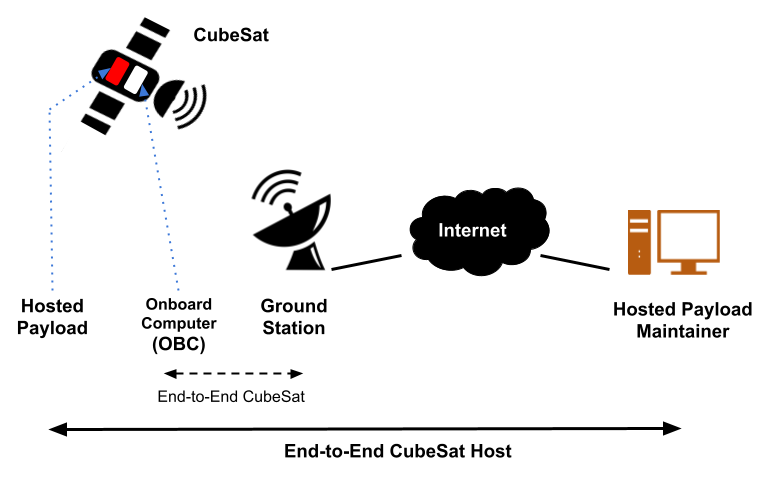
\includegraphics[width=0.4\textwidth]{Figures/CubeSat-Payload-End2End.png}
    \caption{CubeSat hosted payload software update security end-to-end.}
    \label{fig:e2e}
\end{figure}

\subsection*{Paper contributions}
The main contributions of this paper are the following
\begin{itemize}
    \item We provide a case-study, ThingSat: a low-power, low-cost payload hosted on a CubeSat, currently in-orbit;
    \item We analyze its software update requirements and constraints;
    \item We define Cubedate, a generic architecture enabling standards-based, secure software updates for payloads hosted on a low-power CubeSat;
    \item We provide and evaluate an open source implementation of Cubedate.
\end{itemize}
